\documentclass[tikz]{standalone}

\usepackage[utf8]{inputenc}
\usepackage{tikz}
\usetikzlibrary{calc,positioning,fit}
\usepackage{soul}
\usetikzlibrary{snakes}

\begin{document}

\begin{tikzpicture}

\node[draw] (archi_1)
{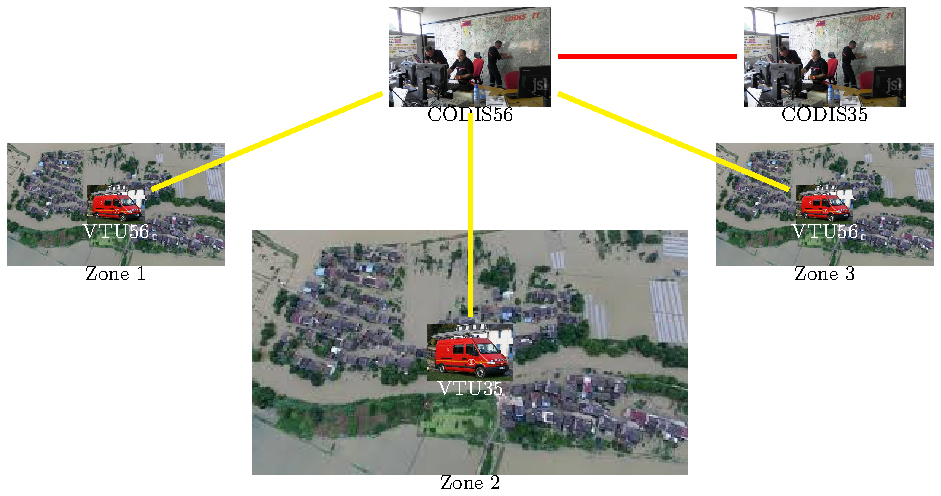
\includegraphics[scale=0.5]{../imgs/fig_overview_conf1.pdf}};

\node[draw, xshift=5cm, above=of archi_1] (archi_2)
{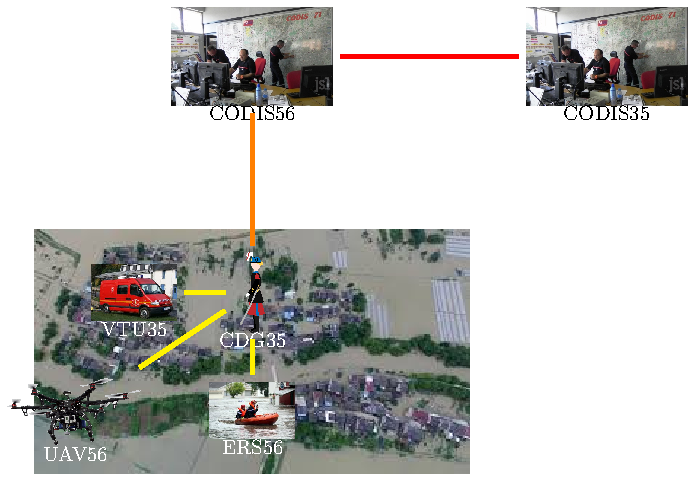
\includegraphics[scale=0.5]{../imgs/fig_overview_conf2.pdf}};

\node[draw, xshift=0.5cm, right=of archi_1] (archi_3)
{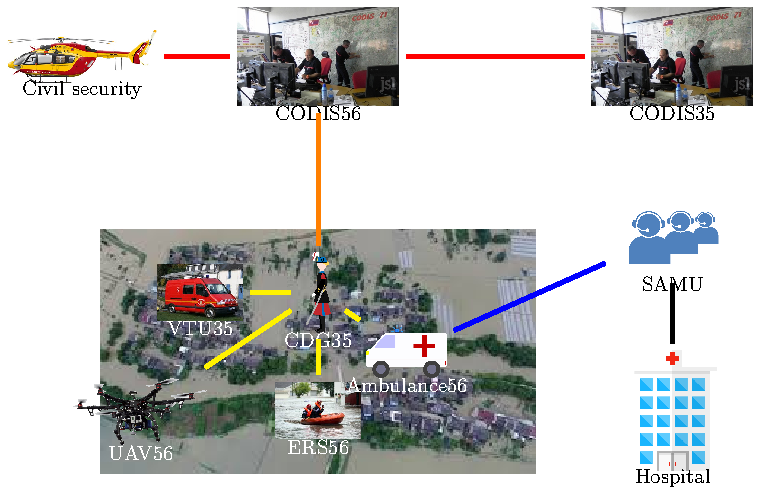
\includegraphics[scale=0.5]{../imgs/fig_overview_conf3.pdf}};
%
\node[yshift=-0.25cm] (label1) at (archi_1.south)
{Collaboration opérationnelle interdep.};

\node[yshift=-0.25cm] (label2) at (archi_2.south)
{Collaboration stratégique interdep.};

\node[yshift=-0.25cm] (label2) at (archi_3.south)
{Collaboration médicale};

\draw[snake=coil, ->] (archi_1) -- (archi_2);
\draw[snake=coil, ->] (archi_2) -- (archi_3);
\end{tikzpicture}



\end{document}
